
% TikZ code for Paper 14 Figure 1: Hierarchical Topology
% Insert this in the LaTeX document

\begin{figure}[t]
\centering
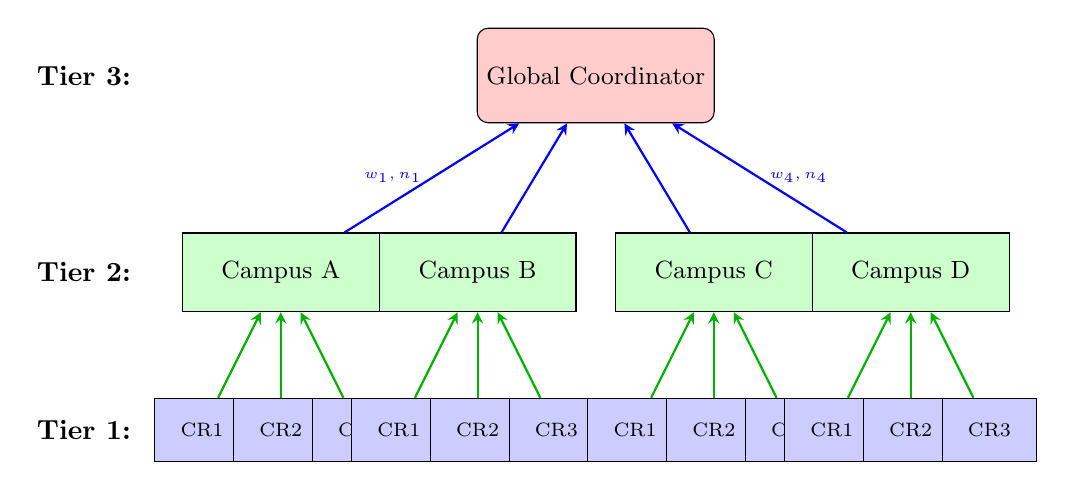
\begin{tikzpicture}[
    node distance=1.2cm,
    edge/.style={->, >=stealth, thick},
    tier1/.style={rectangle, draw, fill=blue!20, minimum width=1.2cm, minimum height=0.8cm, font=\scriptsize},
    tier2/.style={rectangle, draw, fill=green!20, minimum width=2.5cm, minimum height=1cm, font=\small},
    tier3/.style={rectangle, draw, fill=red!20, minimum width=3cm, minimum height=1.2cm, font=\small, rounded corners}
]

% Tier 3: Global Coordinator
\node[tier3] (global) at (0, 0) {Global Coordinator};

% Tier 2: Campus Aggregators
\node[tier2] (campus1) at (-4, -2.5) {Campus A};
\node[tier2] (campus2) at (-1.5, -2.5) {Campus B};
\node[tier2] (campus3) at (1.5, -2.5) {Campus C};
\node[tier2] (campus4) at (4, -2.5) {Campus D};

% Tier 1: Edge Nodes (sample 3 per campus for clarity)
\node[tier1] (e11) at (-5, -4.5) {CR1};
\node[tier1] (e12) at (-4, -4.5) {CR2};
\node[tier1] (e13) at (-3, -4.5) {CR3};

\node[tier1] (e21) at (-2.5, -4.5) {CR1};
\node[tier1] (e22) at (-1.5, -4.5) {CR2};
\node[tier1] (e23) at (-0.5, -4.5) {CR3};

\node[tier1] (e31) at (0.5, -4.5) {CR1};
\node[tier1] (e32) at (1.5, -4.5) {CR2};
\node[tier1] (e33) at (2.5, -4.5) {CR3};

\node[tier1] (e41) at (3, -4.5) {CR1};
\node[tier1] (e42) at (4, -4.5) {CR2};
\node[tier1] (e43) at (5, -4.5) {CR3};

% Connections Tier 2 -> Tier 3
\draw[edge, blue, thick] (campus1) -- (global) node[midway, left, font=\tiny] {$w_1, n_1$};
\draw[edge, blue, thick] (campus2) -- (global);
\draw[edge, blue, thick] (campus3) -- (global);
\draw[edge, blue, thick] (campus4) -- (global) node[midway, right, font=\tiny] {$w_4, n_4$};

% Connections Tier 1 -> Tier 2 (Campus A)
\draw[edge, green!70!black] (e11) -- (campus1);
\draw[edge, green!70!black] (e12) -- (campus1);
\draw[edge, green!70!black] (e13) -- (campus1);

% Campus B
\draw[edge, green!70!black] (e21) -- (campus2);
\draw[edge, green!70!black] (e22) -- (campus2);
\draw[edge, green!70!black] (e23) -- (campus2);

% Campus C
\draw[edge, green!70!black] (e31) -- (campus3);
\draw[edge, green!70!black] (e32) -- (campus3);
\draw[edge, green!70!black] (e33) -- (campus3);

% Campus D
\draw[edge, green!70!black] (e41) -- (campus4);
\draw[edge, green!70!black] (e42) -- (campus4);
\draw[edge, green!70!black] (e43) -- (campus4);

% Labels
\node[font=\small, font=\bfseries] at (-6.5, 0) {Tier 3:};
\node[font=\small, font=\bfseries] at (-6.5, -2.5) {Tier 2:};
\node[font=\small, font=\bfseries] at (-6.5, -4.5) {Tier 1:};

\end{tikzpicture}
\caption{Hierarchical Federated Learning Topology (3-Tier Architecture)}
\label{fig:h_fedavg_topology}
\end{figure}
